\documentclass[a4paper,twocolumn,12pt]{article}
\usepackage[utf8]{inputenc}
\usepackage[MeX]{polski}
\usepackage{fullpage}
\usepackage{tikz}

% ;;;;;;;;; colors ;;;;;;;;;;;;

\definecolor{Board}{RGB}{60,145,143}
\definecolor{DoubleWordBonus}{RGB}{239,174,154}
\definecolor{DoubleLetterBonus}{RGB}{141,201,240}
\definecolor{TripleLetterBonus}{RGB}{54,156,219}
\definecolor{Tile}{RGB}{247,225,190}

% ;;;;;;;;;;;;;;;;;;;;;;;;;;;;;;;;

\title{\LARGE{Sztuczna inteligencja grająca w~Scrabble} \\ \large{Koncepcja implementacji - dane, struktury danych, algorytmy}}
\author{Jakub Turek}
\date{\today}

\begin{document}

\maketitle

\begin{abstract}
Celem artykułu jest opisanie zbioru koncepcji, które posłużą do implementacji algorytmu sztucznej inteligencji grającego w~grę Scrabble w~języku polskim. Artykuł analizuje i~porównuje dane zawarte w~dwóch głównych słownikach wyrazów do gier dla języka polskiego, przedstawia dane statystyczne ułatwiające wprowadzanie heurystyk do algorytmu, a~także opisuje metody niezbędne do wyznaczania wszystkich możliwych kombinacji ruchów w~danej turze. Autor omawia również podział rozgrywki na fazy gry i~przybliża podejście, które pozwala uzyskiwać najlepsze wyniki dla każdej fazy gry.
\end{abstract}

\section*{Wstęp}

Scrabble to ,,gra słowna polegająca na układaniu na określonej planszy wyrazów z~losowanych liter''\footnote{Wielki słownik ortograficzny - PWN 2003, 2006, 2008 - E. Polański}. Jest to bardzo ogólna definicja, którą należy uściślić. Scrabble jest grą przeznaczoną dla 2-4 osób. Akcesoriami do gry są: kwadratowa plansza o~stałym rozmiarze $15 \times 15$, torebka wypełniona płytkami, na których nadrukowane są litery oraz ich wartości punktowe, a~także stojaki, na których gracze umieszczają płytki, którymi w~danej chwili dysponują.

Gra rozgrywana jest w~turach. Zadaniem graczy jest układanie wyrazów na planszy, w~taki sposób aby tworzyły one poprawne słowa w~języku, w~którym prowadzona jest rozgrywka, w~układzie krzyżówkowym. Układ krzyżówkowy został przedstawiony na rysunkach \ref{fig:crossword_first} oraz \ref{fig:crossword_second}:

\begin{description}
 \item [Rysunek \ref{fig:crossword_first}] Pokazuje sytuację początkową obrazującą pewien moment rozgrywki.
 \item [Rysunek \ref{fig:crossword_second}] Pokazuje poprawny ruch zawodnika, który powoduje powstanie więcej niż jednego słowa. Wszystkie wyrazy utworzone przez jeden ruch muszą być poprawne. W~podanym przykładzie słowa ,,za'' i~,,masz'' są poprawne.
\end{description}

\begin{figure}[ht!]
	\begin{center}
			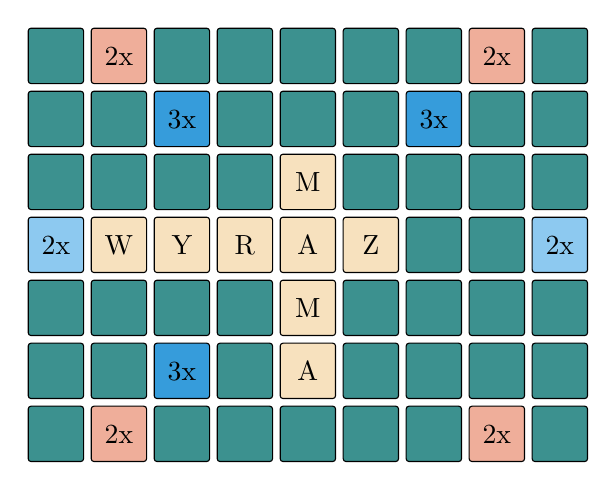
\begin{tikzpicture}
			\tikzstyle{every node}=[draw, shape=rectangle, rounded corners = 1pt, minimum width = 20pt, minimum height = 20pt, align=center, text height = 7pt];
			\node [fill=Board] at (-0.8, 0) {};
			\node [fill=DoubleWordBonus] at (0, 0) {2x};
			\node [fill=Board] at (0.8, 0) {};
			\node [fill=Board] at (1.6, 0) {};
			\node [fill=Board] at (2.4, 0) {};
			\node [fill=Board] at (3.2, 0) {};
			\node [fill=Board] at (4.0, 0) {};
			\node [fill=DoubleWordBonus] at (4.8, 0) {2x};
			\node [fill=Board] at (5.6, 0) {};
			\node [fill=Board] at (-.8, -.8) {};
			\node [fill=Board] at (0, -.8) {};
			\node [fill=TripleLetterBonus] at (0.8, -.8) {3x};
			\node [fill=Board] at (1.6, -.8) {};
			\node [fill=Board] at (2.4, -.8) {};
			\node [fill=Board] at (3.2, -.8) {};
			\node [fill=TripleLetterBonus] at (4.0, -.8) {3x};
			\node [fill=Board] at (4.8, -.8) {};
			\node [fill=Board] at (5.6, -.8) {};
			\node [fill=Board] at (-.8, -1.6) {};
			\node [fill=Board] at (0, -1.6) {};
			\node [fill=Board] at (0.8, -1.6) {};
			\node [fill=Board] at (1.6, -1.6) {};
			\node [fill=Tile] at (2.4, -1.6) {M};
			\node [fill=Board] at (3.2, -1.6) {};
			\node [fill=Board] at (4.0, -1.6) {};
			\node [fill=Board] at (4.8, -1.6) {};
			\node [fill=Board] at (5.6, -1.6) {};
			\node [fill=DoubleLetterBonus] at (-.8, -2.4) {2x};
			\node [fill=Tile] at (0, -2.4) {W};
			\node [fill=Tile] at (.8, -2.4) {Y};
			\node [fill=Tile] at (1.6, -2.4) {R};
			\node [fill=Tile] at (2.4, -2.4) {A};
			\node [fill=Tile] at (3.2, -2.4) {Z};
			\node [fill=Board] at (4.0, -2.4) {};
			\node [fill=Board] at (4.8, -2.4) {};
			\node [fill=DoubleLetterBonus] at (5.6, -2.4) {2x};
			\node [fill=Board] at (-.8, -3.2) {};
			\node [fill=Board] at (0, -3.2) {};
			\node [fill=Board] at (0.8, -3.2) {};
			\node [fill=Board] at (1.6, -3.2) {};
			\node [fill=Tile] at (2.4, -3.2) {M};
			\node [fill=Board] at (3.2, -3.2) {};
			\node [fill=Board] at (4.0, -3.2) {};
			\node [fill=Board] at (4.8, -3.2) {};
			\node [fill=Board] at (5.6, -3.2) {};
			\node [fill=Board] at (-.8, -4.0) {};
			\node [fill=Board] at (0, -4.0) {};
			\node [fill=TripleLetterBonus] at (0.8, -4.0) {3x};
			\node [fill=Board] at (1.6, -4.0) {};
			\node [fill=Tile] at (2.4, -4.0) {A};
			\node [fill=Board] at (3.2, -4.0) {};
			\node [fill=Board] at (4.0, -4.0) {};
			\node [fill=Board] at (4.8, -4.0) {};
			\node [fill=Board] at (5.6, -4.0) {};
			\node [fill=Board] at (-.8, -4.8) {};
			\node [fill=DoubleWordBonus] at (0, -4.8) {2x};
			\node [fill=Board] at (0.8, -4.8) {};
			\node [fill=Board] at (1.6, -4.8) {};
			\node [fill=Board] at (2.4, -4.8) {};
			\node [fill=Board] at (3.2, -4.8) {};
			\node [fill=Board] at (4.0, -4.8) {};
			\node [fill=DoubleWordBonus] at (4.8, -4.8) {2x};
			\node [fill=Board] at (5.6, -4.8) {};
		\end{tikzpicture}
		\caption{Fragment planszy. Gracze ułożyli kolejno słowa: ,,wyraz'' oraz ''mama''.}
		\label{fig:crossword_first}
	\end{center}
\end{figure}

\begin{figure}[ht!]
	\begin{center}
			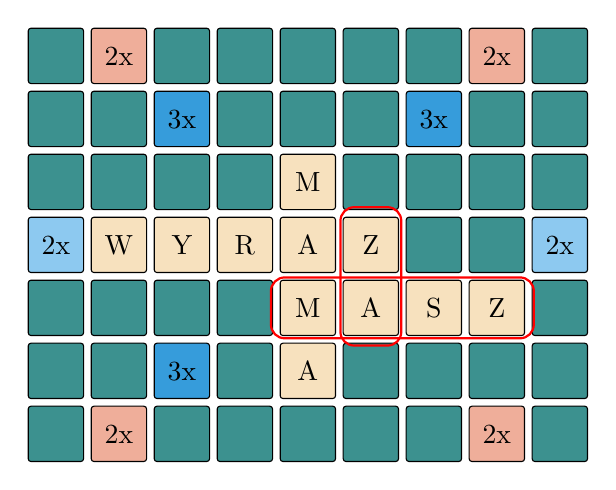
\begin{tikzpicture}
			\tikzstyle{every node}=[draw, shape=rectangle, rounded corners = 1pt, minimum width = 20pt, minimum height = 20pt, align=center, text height = 7pt];
			\node [fill=Board] at (-0.8, 0) {};
			\node [fill=DoubleWordBonus] at (0, 0) {2x};
			\node [fill=Board] at (0.8, 0) {};
			\node [fill=Board] at (1.6, 0) {};
			\node [fill=Board] at (2.4, 0) {};
			\node [fill=Board] at (3.2, 0) {};
			\node [fill=Board] at (4.0, 0) {};
			\node [fill=DoubleWordBonus] at (4.8, 0) {2x};
			\node [fill=Board] at (5.6, 0) {};
			\node [fill=Board] at (-.8, -.8) {};
			\node [fill=Board] at (0, -.8) {};
			\node [fill=TripleLetterBonus] at (0.8, -.8) {3x};
			\node [fill=Board] at (1.6, -.8) {};
			\node [fill=Board] at (2.4, -.8) {};
			\node [fill=Board] at (3.2, -.8) {};
			\node [fill=TripleLetterBonus] at (4.0, -.8) {3x};
			\node [fill=Board] at (4.8, -.8) {};
			\node [fill=Board] at (5.6, -.8) {};
			\node [fill=Board] at (-.8, -1.6) {};
			\node [fill=Board] at (0, -1.6) {};
			\node [fill=Board] at (0.8, -1.6) {};
			\node [fill=Board] at (1.6, -1.6) {};
			\node [fill=Tile] at (2.4, -1.6) {M};
			\node [fill=Board] at (3.2, -1.6) {};
			\node [fill=Board] at (4.0, -1.6) {};
			\node [fill=Board] at (4.8, -1.6) {};
			\node [fill=Board] at (5.6, -1.6) {};
			\node [fill=DoubleLetterBonus] at (-.8, -2.4) {2x};
			\node [fill=Tile] at (0, -2.4) {W};
			\node [fill=Tile] at (.8, -2.4) {Y};
			\node [fill=Tile] at (1.6, -2.4) {R};
			\node [fill=Tile] at (2.4, -2.4) {A};
			\node [fill=Tile] at (3.2, -2.4) {Z};
			\node [fill=Board] at (4.0, -2.4) {};
			\node [fill=Board] at (4.8, -2.4) {};
			\node [fill=DoubleLetterBonus] at (5.6, -2.4) {2x};
			\node [fill=Board] at (-.8, -3.2) {};
			\node [fill=Board] at (0, -3.2) {};
			\node [fill=Board] at (0.8, -3.2) {};
			\node [fill=Board] at (1.6, -3.2) {};
			\node [fill=Tile] at (2.4, -3.2) {M};
			\node [fill=Tile] at (3.2, -3.2) {A};
			\node [fill=Tile] at (4.0, -3.2) {S};
			\node [fill=Tile] at (4.8, -3.2) {Z};
			\node [fill=Board] at (5.6, -3.2) {};
			\node [fill=Board] at (-.8, -4.0) {};
			\node [fill=Board] at (0, -4.0) {};
			\node [fill=TripleLetterBonus] at (0.8, -4.0) {3x};
			\node [fill=Board] at (1.6, -4.0) {};
			\node [fill=Tile] at (2.4, -4.0) {A};
			\node [fill=Board] at (3.2, -4.0) {};
			\node [fill=Board] at (4.0, -4.0) {};
			\node [fill=Board] at (4.8, -4.0) {};
			\node [fill=Board] at (5.6, -4.0) {};
			\node [fill=Board] at (-.8, -4.8) {};
			\node [fill=DoubleWordBonus] at (0, -4.8) {2x};
			\node [fill=Board] at (0.8, -4.8) {};
			\node [fill=Board] at (1.6, -4.8) {};
			\node [fill=Board] at (2.4, -4.8) {};
			\node [fill=Board] at (3.2, -4.8) {};
			\node [fill=Board] at (4.0, -4.8) {};
			\node [fill=DoubleWordBonus] at (4.8, -4.8) {2x};
			\node [fill=Board] at (5.6, -4.8) {};
			\node [draw, thick, shape = rectangle, rounded corners = 5pt, color = red, fill = none, minimum height = 22 pt, minimum width = 95 pt] at (3.6, -3.2) {};
			\node [draw, thick, shape = rectangle, rounded corners = 5pt, color = red, fill = none, minimum width = 22 pt, minimum height = 50 pt] at (3.2, -2.8) {};
		\end{tikzpicture}
		\caption{Fragment planszy. Ruch przez dołożenie liter A, S, Z tworzy dwa wyrazy w~układzie krzyżówkowym.}
		\label{fig:crossword_second}
	\end{center}
\end{figure}

W~trakcie jednego ruchu zawodnik może układać płytki tylko w~jednym kierunku (pionowo lub poziomo). Utworzony przez zawodnika wyraz musi być spójny, to znaczy, że wszystkie płytki muszą przylegać do siebie bezpośrednio lub poprzez płytki już istniejące na planszy. Wymagane jest, aby tworzone słowo przylegało do przynajmniej jednej płytki, która jest już umieszczona na planszy (nie dotyczy to pierwszego ruchu).

Punktacja za dane zagranie jest obliczana jako suma punktów za wszystkie płytki, które wchodzą w~skład utworzonych wyrazów (a~więc również tych, które przed zagraniem znajdowały się na planszy), z~uwzględnieniem niewykorzystanych premii wynikających z~pozycji płytki na planszy:

\begin{description}
 \item [Premia literowa] Podwaja lub potraja wartość danej płytki.
 \item [Premia słowna] Podwaja lub potraja wartość całego wyrazu.
\end{description}



\end{document}
